

\chapter{Analytics}
\label{Analytics}

Ziel: Analyse von Twitterdaten

Live analytics und offline batch analytics bla.
\TODO{Some Goalgs to be defined bla}

\begin{figure}[H]
	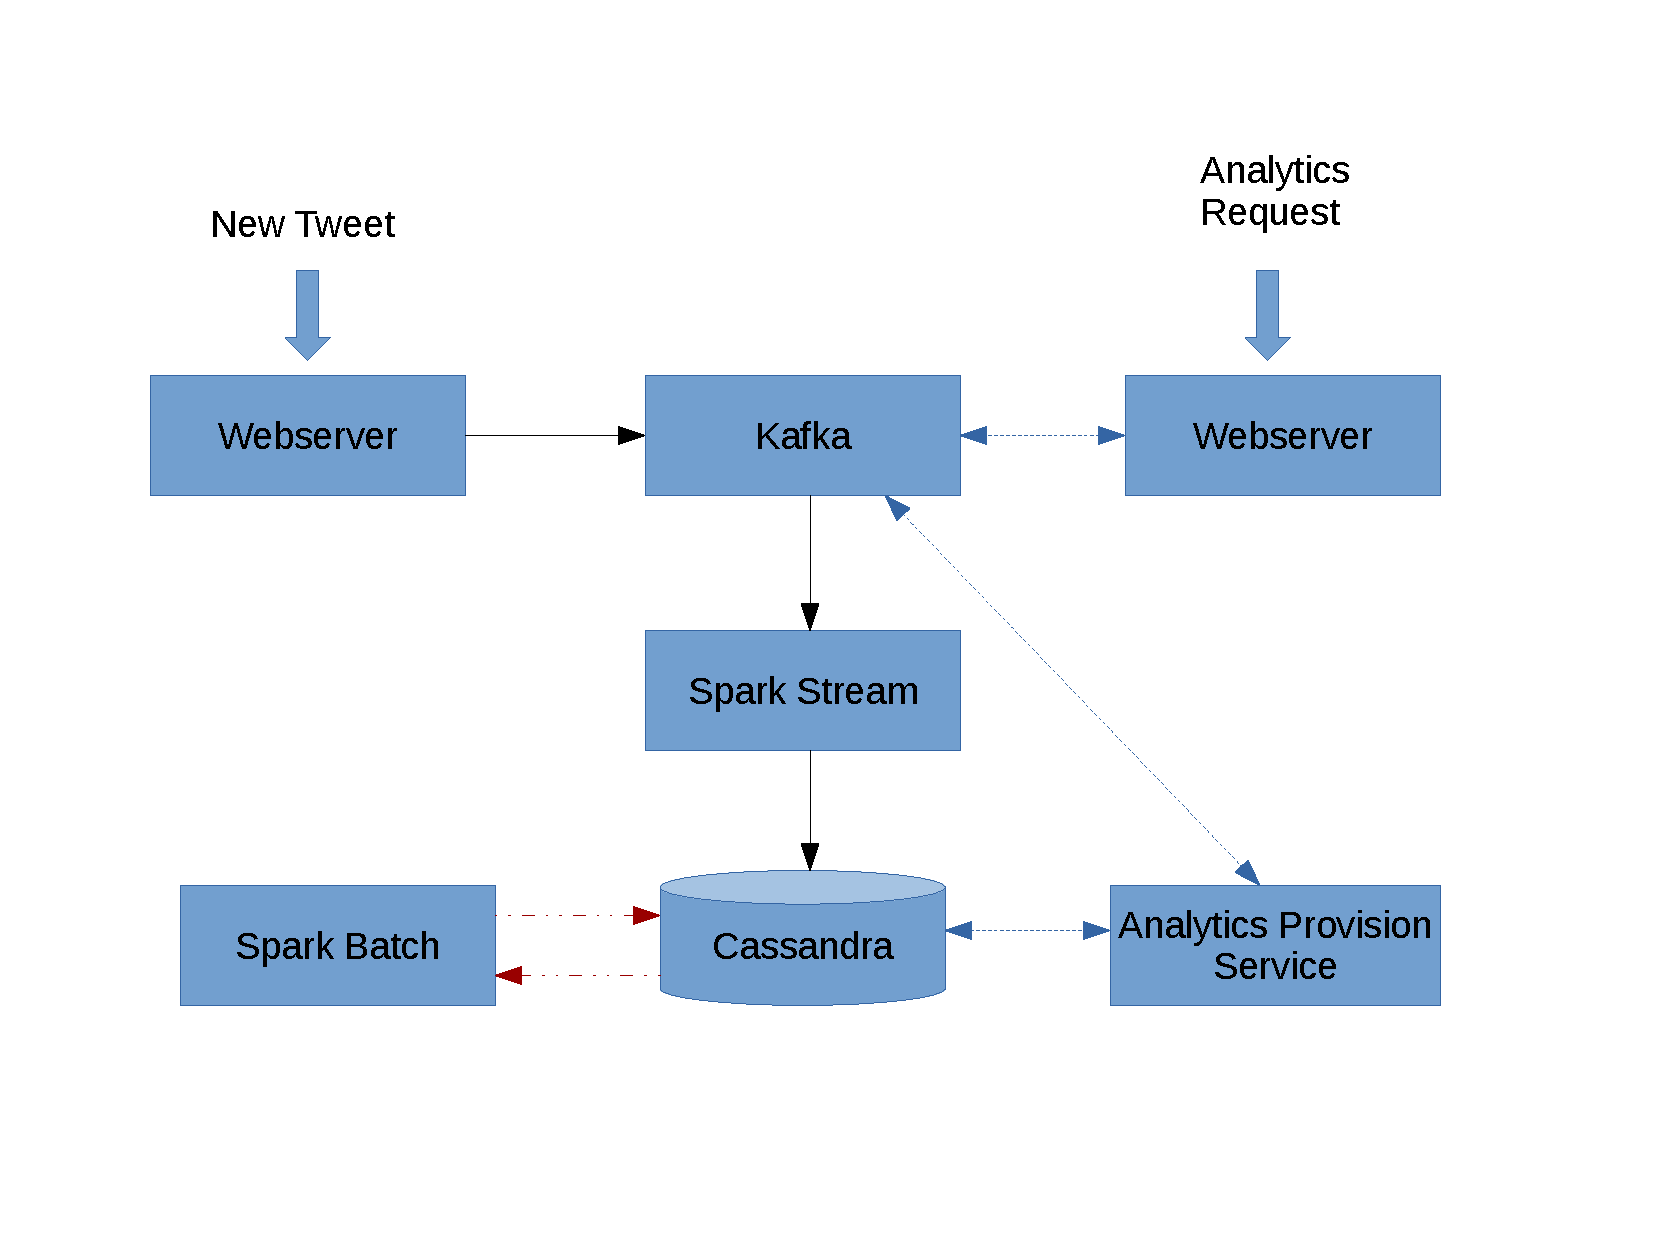
\includegraphics[width=\textwidth]{pics/analytics/archi}
	\caption{Übersicht der Analytics Komponenten}
\end{figure}

\section{Stream}

Die Streamverarbeitung innerhalb des Hamaube-Systems ist als eigenständiger Service geschrieben. Für die Umsetzung wurde SparkStreaming im Verbund mit Scala verwendet.

Folgende Ziele haben sich während des Projekt herausgebildet:
\begin{itemize}
	\item Vorverarbeitung der eingehenden Tweets für eine spätere Prozessierung mittels Spark
	\item Verarbeitung der Streamdaten für live Analyseergebnisse.
\end{itemize}


Als Input dienen bisher die beiden gegebenen Datenquellen:
\begin{enumerate}
	\item Tweets, welche aus der Twitter API in unsere Anwendung gestreamt werden.
	\item Hamaube-Tweets, welche in unserer Anwendung erzeugt werden.
\end{enumerate}

Auch die Streamverarbeitung ist über Kafka angebunden und erhält die Tweets über das \textit{USER\_ISSUES\_TWEET} Topic.


\subsection*{Vorverarbeitung für Spark Batch Processing}
Aus verschiedenen Gründen wurde für die Tweets im Hamaube-System das Datenmodell von Twitter übernommen.
Dadurch enthalten Tweets (vorallem solche, die direkt von Twitter kommen) eine Vielzahl von nicht gesetzten Feldern oder Daten, welche für die Analyse wenig interessant sind.
In der Vorverarbeitung wird nur ein definierter Teil der Felder eines Tweets übernommen und der Rest verworfen.
Zusätzlich werden (sofern vorhanden) die im Tweet enthaltenen Hashtags extrahiert und neben dem eigentlichen Tweet gespeichert.
Außerdem wird anhand des Tweet-Textes eine Sentiment Analyse durchgeführt, welche dem Tweet einen Score zuordnet, der dessen Stimmung wiederspiegelt (negativ - negative Stimmung, positiv - positive Stimmung). Auch dieser Score wird neben dem eigentlichen Tweet gespeichert.

Wir haben uns dazu entschieden, die Tweetdaten zusätzlich - also dupliziert - zu den schon gespeicherten Tweets des 'CassandraReaders' in Cassandra zu speichern, da wir in Hinsicht auf ein produktives System die kritischen Tabellen nicht zusätzlich mit Anfragen belasten wollen.
Für die Analyse würde also ein separate Umgebung für Cassandra aufgebaut, dies haben im Hamaube-System aufgrund der Einfachheit noch nicht umgesetzt.

\subsection*{Live Analyse}
Zudem wird auf den durch Kafka eingehenden Tweetstream eine Live Analyse durchgeführt.
Das Spark Streaming Framework teilt den Stream dafür in Micro-Batches, die dann weiter verarbeitet werden können.
So werden z.B. die Anzahl von Hashtag pro Stunde/pro Minute ermittelt, daraus werden dann aktuell beliebte Hashtags erkannt.
Auch diese Ergebnisse werden in Cassandra gespeichert.
Um eine Skalierungs zu ermöglichen müssen die Ergebnisse z.B. pro Stunde von mehreren Instanzen geupdated werden können, ohne dass dabei dirty reads oder Überschreibungen auftreten dürfen. Cassandra bietet hier den Datentyp \textbf{Counter}, der atomare \textit{increase} und \textit{decrease} Operationen anbietet. Damit lassen sich die meisten Szenarien realisieren, ohne weitere  komplexe (und möglicherweise verlangsamende) Isolierungsmechaniken zu implementieren.

\begin{figure}[h]
\centering
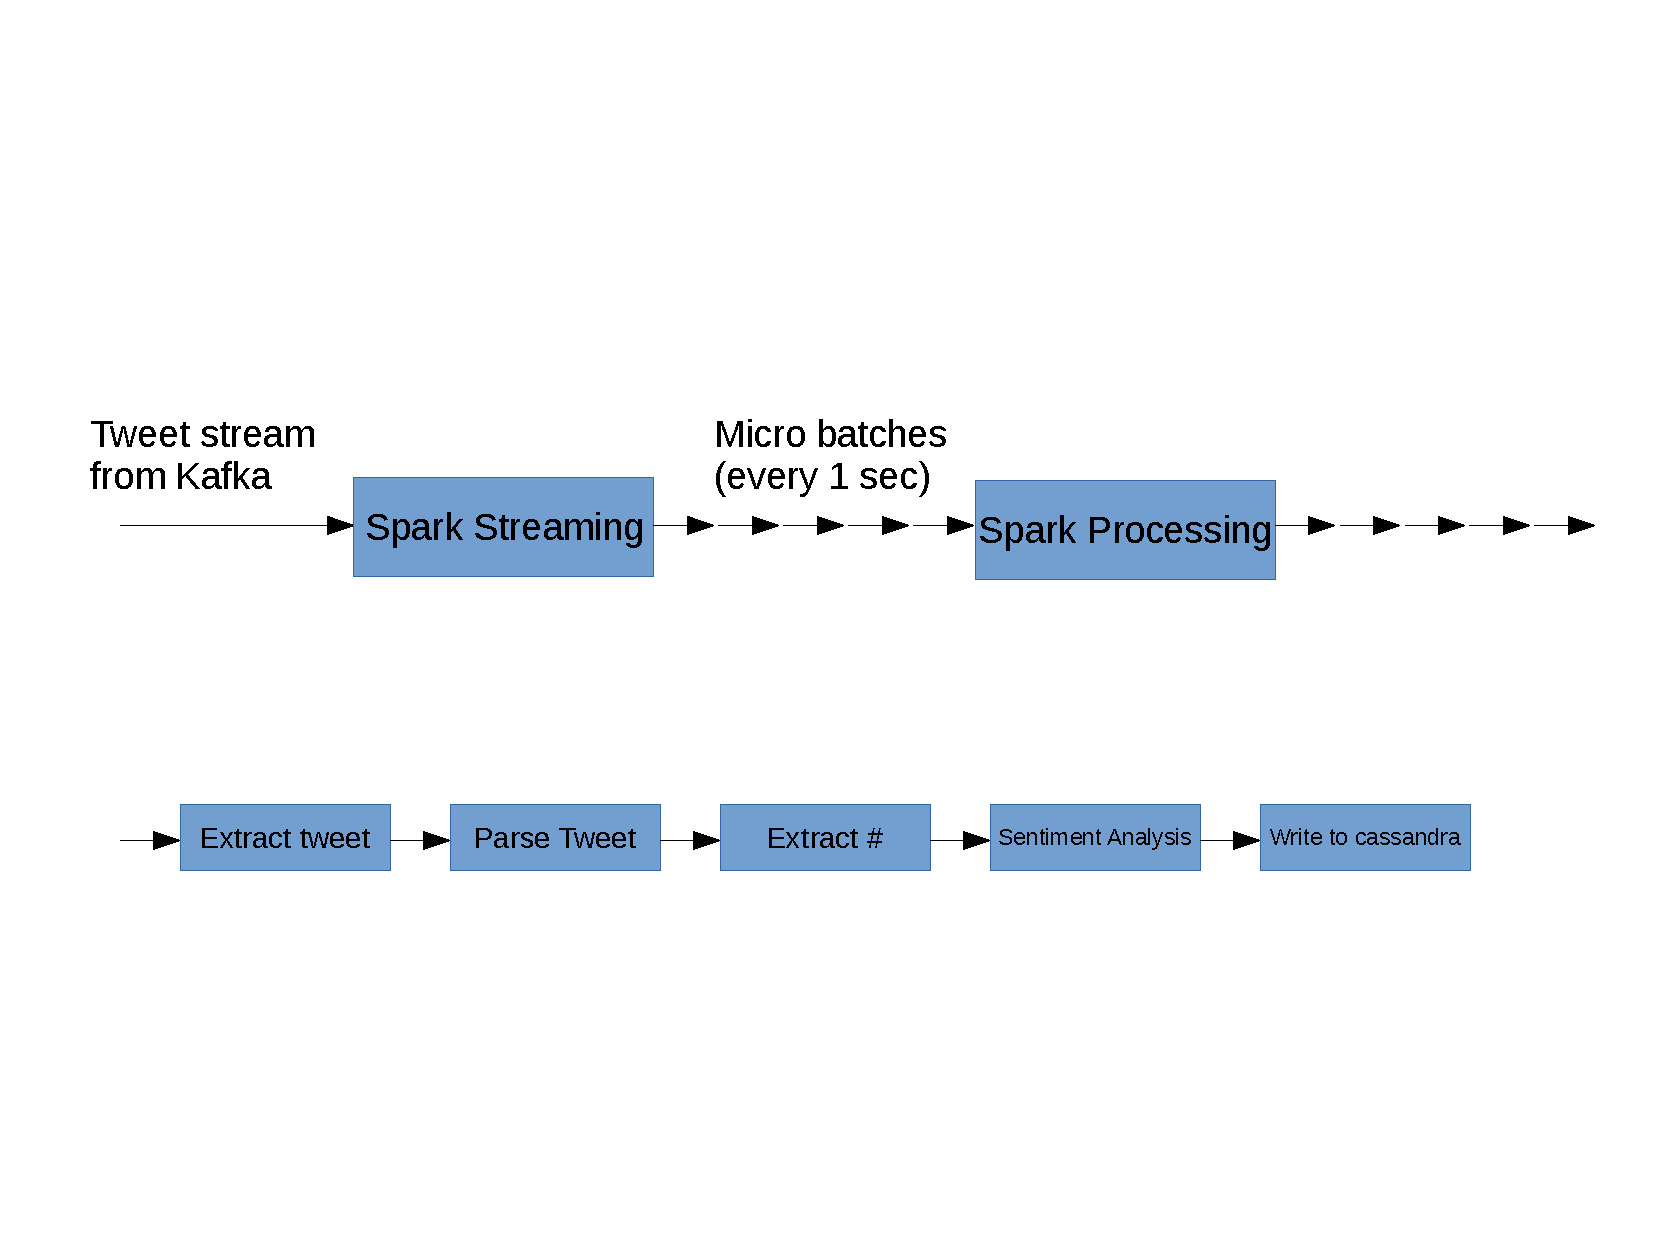
\includegraphics[width=\linewidth]{../Bericht/streamProcessing}
\caption{Spark stream processing}
\label{fig:streamProcessing}
\end{figure}





\section{Batch}

....

\TODO{TO BE MERGED}


\section{Analytics Provisioning Service}

Für die Bereitstellung der Analysedaten ist der Micro Service \textit{Analytics Provisioning Service} zuständig. 
Dieser liest auf Anfrage Analysedaten aus Cassandra und bereitet diese für die Darstellung im Frontend auf.
In Batchanalyse werden die Ergebnisse geordnet in einer Tabelle pro Analyse gelegt, diese werden einfach nur für die letzten 14 Tage gelesen. Ergebnisse, die weiter in der Vergangenheit liegen, werden zur Zeit nicht bereit gestellt, dies ist theoretisch aber möglich.
Da Cassandra keine Counter als sekundäre Keys unterstützt und nicht für Sortierungen von großen Datenmengen ausgelegt ist,
die Analysedaten aus dem Stream jedoch unsortiert und nicht gefiltert vorliegen, war der naive Ansatz diese mittels einer  user-defined function in Cassandra pro Anfrage zu sortieren. Dies ist aber mit steigenden Tweetzahlen sehr aufwändig und könnte z.B. durch weitere Umsetzungen mit Spark ersetzt werden.

Die Kommunikation passiert auch hier über Kafka und festgelegte Topics.
Es lassen sich beliebig viele Instanzen des Services starten, die Kommunikation skaliert automatisch über die gewählte Kommunikationsarchitektur.

Für die Umsetzung wurde die Platform Node.js mit TypeScrict verwendet. 